\documentclass[letterpaper,12pt]{article}

\usepackage{threeparttable}
\usepackage{geometry}
\geometry{letterpaper,tmargin=1in,bmargin=1in,lmargin=1.25in,rmargin=1.25in}
\usepackage[format=hang,font=normalsize,labelfont=bf]{caption}
\usepackage{amsmath}
\usepackage{multirow}
\usepackage{array}
\usepackage{delarray}
\usepackage{amssymb}
\usepackage{amsthm}
\usepackage{lscape}
\usepackage[round]{natbib}
\usepackage{setspace}
\usepackage{float,color}
\usepackage[pdftex]{graphicx}
\usepackage{pdfsync}
\usepackage{verbatim}
\usepackage{placeins}
\usepackage{geometry}
\usepackage{pdflscape}
\synctex=1
\usepackage{hyperref}
\hypersetup{colorlinks,linkcolor=red,urlcolor=blue,citecolor=red}
\usepackage{bm}
\usepackage{tabu}

\theoremstyle{definition}
\newtheorem{theorem}{Theorem}
\newtheorem{acknowledgement}[theorem]{Acknowledgement}
\newtheorem{algorithm}[theorem]{Algorithm}
\newtheorem{axiom}[theorem]{Axiom}
\newtheorem{case}[theorem]{Case}
\newtheorem{claim}[theorem]{Claim}
\newtheorem{conclusion}[theorem]{Conclusion}
\newtheorem{condition}[theorem]{Condition}
\newtheorem{conjecture}[theorem]{Conjecture}
\newtheorem{corollary}[theorem]{Corollary}
\newtheorem{criterion}[theorem]{Criterion}
\newtheorem{definition}{Definition} % Number definitions on their own
\newtheorem{derivation}{Derivation} % Number derivations on their own
\newtheorem{example}[theorem]{Example}
\newtheorem{exercise}[theorem]{Exercise}
\newtheorem{lemma}[theorem]{Lemma}
\newtheorem{notation}[theorem]{Notation}
\newtheorem{problem}[theorem]{Problem}
\newtheorem{proposition}{Proposition} % Number propositions on their own
\newtheorem{remark}[theorem]{Remark}
\newtheorem{solution}[theorem]{Solution}
\newtheorem{summary}[theorem]{Summary}
\bibliographystyle{aer}
\newcommand\ve{\varepsilon}
\renewcommand\theenumi{\roman{enumi}}
\newcommand\norm[1]{\left\lVert#1\right\rVert}

\begin{document}

\begin{titlepage}
\title{Evaluating A Markov Regime-switching Model of Health Care Expenditure Dynamics \thanks{This paper is a final project for Structural Estimation course in Winter Quarter 2017 at the University of Chicago. We express our sincerest gratitude to the course instructor Dr. James W. Evans for his guidance and support. We are especially thankful to Dr. Evans for allowing us to use his original research project and data to complete the current paper.}
       }
       \author{
  Bobae Kang\footnote{The University of Chicago, MA Program in the Social Science, \href{mailto:bobaekang@uchicago.edu}{bobaekang@uchicago.edu}.} \\[-2pt]
  \and
  Dongping Zhang\footnote{The University of Chicago, MA in Computational Social Science, \href{mailto:dpzhang@uchicago.edu}{dpzhang@uchicago.edu}.}}
\date{March 2017 \\
  \scriptsize{(version 17.03.a)}}
\maketitle
\vspace{-9mm}
\begin{abstract}
\small{This paper replicates and evaluates a Markov regime-switching approach to estimating the dynamic process of health care expenditure proposed by \citet{evans}. Our data includes the recorded monthly health expenditure of 99,965 individuals for 24-month period. The model assumes five distinct health-care-consumption states, among which two are zero-expenditure states and the rest of three are positive-expenditure states. The model also assumes that the proportion of the given population in those five health states is a ergodic dynamical system. We use GMM to estimate the Markov model parameters and have successfully matched target moments. We then label each string of consecutive positive health spending as one of the three positive-expenditure states. We examine the labeled positive-expenditure spells empirically and suggest an alternative labeling scheme to better characterize each health-care-consumption state.
\vspace{3mm}

\noindent\textit{keywords:}\: Heath care expenditure, Markov chain, Markov regime-switching model.

\vspace{3mm}
}

\end{abstract}
\thispagestyle{empty}
\end{titlepage}


\begin{spacing}{1.5}{}

\section{Introduction}\label{SecIntro}

  \citet*{evans} offers a Markov regime-switching model for estimating and simulating monthly health care expenditures of individuals given their current health state. \citet{evans} contrasts their Markov model to the stochastic variance model of \citet{french}, which models the process for log health costs as ``the sum of a white noise process and a highly persistent AR(1) process'' with catastrophic health cost shocks. The Markov regime-switch approach to health expenditures, \citet{evans} argues, has at least two following advantages. First, it better accounts for the prevalence zero-expenditure periods. Second, the Markov process is more appealing on the intuitive level as it allows for clear distinction between different health states wherein ``healthy'' state is subdivided into two categories and ``unhealthy'' into three.\par
  
  In this paper, we replicate the Markov regime-switching model for estimating health care costs by \citet{evans} to validate and evaluate the effectiveness of the model. We use the same data used by the original study but with minor adjustment. We follow the steps provided by the original study to estimate the health care expenditure process. Moreover, we consider extra dimensions of gender and age, which are mostly disregarded in the original study, to enrich our understanding of the characteristics of distinct health expenditure categories. Our examination illustrates that gender and age can provide additional information about different types of positive health expenditure. We further suggest that the labels for health care expenditure types in \citet{evans} may not fully capture the key features of some positive expenditure types, and would like to propose an alternative labeling scheme.\par 
   
  The structure of the rest of this paper is as follows. Section \ref{SecData} describes the data used to estimate the model. Section \ref{SecModel} describes the Markov model used in this paper. Section \ref{SecEstimation} consists of two parts. Part \ref{SecEstimation1} describes the GMM estimation procedure used to estimate model parameters and to present the estimation results. Part \ref{SecEstimation2} describes and discusses the process of identifying positive health expenditure types. Section \ref{SecConclusion} provides a brief conclusion of this paper.  


\section{Data}\label{SecData}

    We estimate the parameters of our model using a panel of total monthly health care expenditures for the same 24-month periods from a random sample of 99,965 individuals residing in the same U.S. city. In addition to their health expenditures, we would also include individual characteristics, such as age and gender, into our analysis.\footnote{Original data set included approximately 102,000 individuals and thus around 240,000 total recorded monthly health expenditures, among which 37 individuals have negative monthly health expenditures. As in \citet{evans}, we excluded 35 individuals from our truncated data set with negative monthly expenditures and only used the remaining for the estimation of our model.} Our data set consists of a subset of the monthly health care expenditures data used in \citet{evans}, with minor adjustments to prevent identifications of the individuals as well as the insurer. Following \citet{evans}, we assume a low degree of elasticity in the demand for health care, which provides a justification for using the health care expenditures as a proxy to predict actual health status.\par
  
  \begin{table}[h!] \centering \captionsetup{width=4.0in}
    \caption{\label{TabDesciprtive}\textbf{Descriptive statistics of the monthly health care expenditures}}
      \begin{tabular}{ c c | c  c  c  c  c  c }
      \hline\hline
        & & Count & Mean & Median & Max & Min & St. Dev. \\
      \hline
      Expenditure & Total & 2,399,160 & 305.31 & 0.0 & 422,855.84 & 0.0 & 2,235.93 \\
       & Zero & 1,375,975 & - & - & - & - & - \\
       & Positive & 1,023,185 & 715.88 & 173.30 & 422,855.84 & 0.01 & 3,380.62 \\
       & Female & 1,228,872 & 328.18 & 0.0 & 355,495.02 & 0.0 & 2,008.85 \\
       & Male & 1,170,288 & 281.29 & 0.0 & 422,855.84 & 0.0 & 2,451.61 \\
      \hline
      Age & total & 99,965 & 33.20 & 36 & 95 & 0 & 18.45 \\
       & Female & 51,203 & 33.30 & 36 & 94 & 0 & 18.18 \\
       & Male & 48,762 & 33.09 & 36 & 95 & 0 & 18.73 \\
      \hline\hline
    \end{tabular}
    % \begin{tablenotes}
    %   \scriptsize{\item[]Note: Maybe put sources here.}
    % \end{tablenotes}
  \end{table}    

  Table \ref{TabDesciprtive} provides a detailed descriptive statistics of our data. As in \citet{evans}, the most outstanding characteristic of the data is that more than half of our total observations (57.35\%) have zero expenditures. As \citet{evans} points out, such prevalence of zero-expenditure months poses a challenge to estimate monthly spending with a stochastic variance model. Figure \ref{FigZeroExpMonths} is a histogram that provides more details about the distribution of the zero-expenditure months. For example, over one-eighth of all individuals, which constitute the largest group of all, have spent nothing for the entire span of 24 months. On the other hand, the second largest group, which accounts for nearly 8\% of all individuals, consists of those with positive expenditures during the entire 24-months period. The rest of the groups takes between 2\% and 5\% of the entire sample.\par
  
  \begin{figure}[h!]\centering \captionsetup{width=4.0in}
    \caption{\label{FigZeroExpMonths}\textbf{Histogram of the fraction of individuals with a given number of zero-expenditure months}}
    \fbox{\resizebox{4.0in}{2.7in}{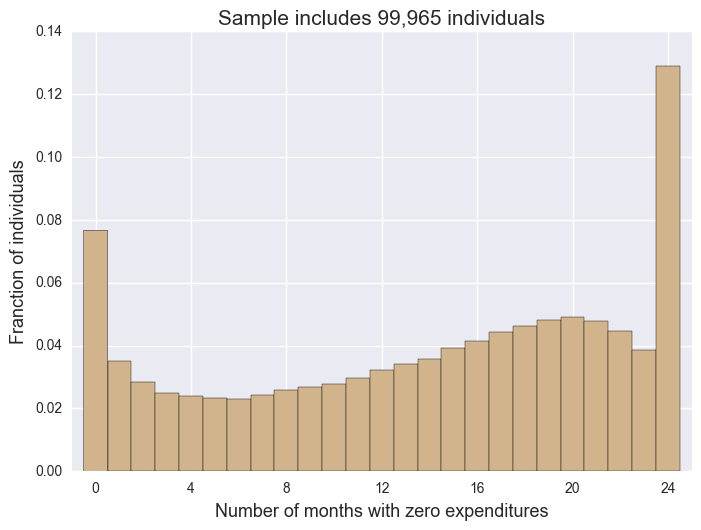
\includegraphics{images/fig_3}}}
  \end{figure}

  Figure \ref{FigPosExpMonths1} illustrates the mean and the standard deviation of positive health care expenditures by month. Although the mean of all positive monthly expenditure shows little change over the 24-month period, the standard deviation varies much more noticeable from one month to another. Perhaps the more informative is Figure \ref{FigPosExpMonths2}, which shows the mean and the standard deviation of individuals by number of months when they have positive health care spending. There is a positive correlation between the number of positive-expenditure months and averaged monthly expenditures. In other words, people who commit to monthly health care frequently would typically have greater health care expenditures per month on average.\par 
 
   \begin{figure}[h!]\centering\captionsetup{width=4.0in}
    \caption{\label{FigPosExpMonths1}\textbf{Mean and standard deviation of positive monthly expenditures by month}}
    \fbox{\resizebox{4.0in}{2.7in}{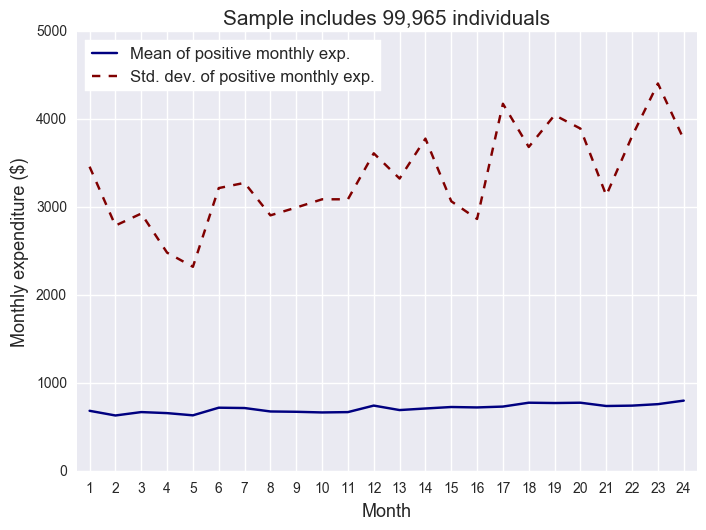
\includegraphics{images/fig_1}}}
  \end{figure}
  
  \begin{figure}[h!]\centering\captionsetup{width=4.0in}
    \caption{\label{FigPosExpMonths2}\textbf{Mean and standard deviation of positive monthly expenditures for individuals by number of positive expenditure months}}
    \fbox{\resizebox{4.0in}{2.7in}{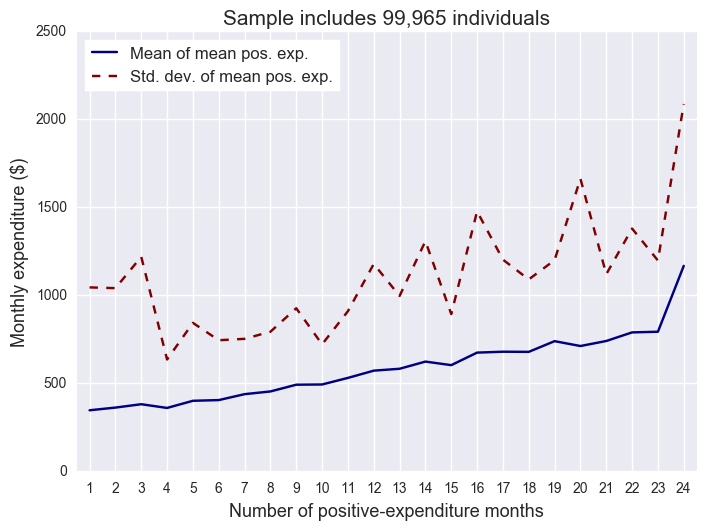
\includegraphics{images/fig_2}}}
  \end{figure} 

  Gender is almost equally divided between female (51.2\%) and male (48.8\%) in our data. On average, female individuals have higher monthly health expenditures than their male counterparts, but the one with the highest monthly spending is a male. Figure \ref{FigGenderAgeDist} illustrates the age distribution of individuals by gender. For both female and male individuals, the age is distributed in a bimodal fashion with the first peak in late teenage hood and the second peak around the late-40s and early-50s.\par

  \begin{figure}[h!]\centering \captionsetup{width=4.0in}
    \caption{\label{FigGenderAgeDist}\textbf{The distribution of male and female individuals by age}}
    \fbox{\resizebox{4.0in}{3.0in}{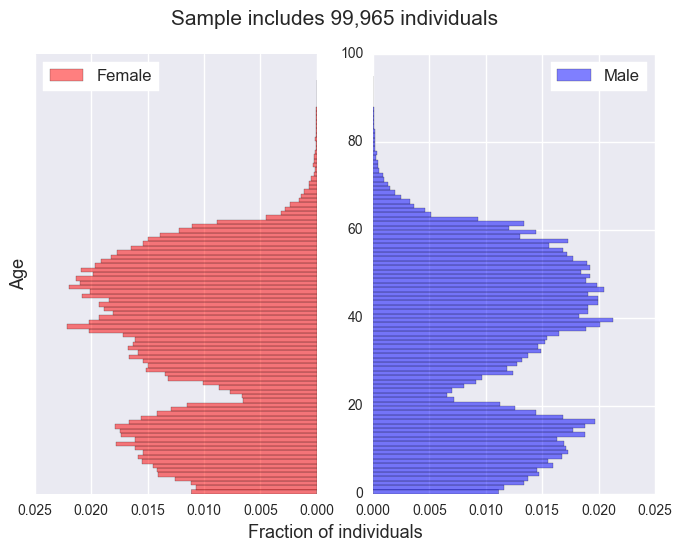
\includegraphics{images/fig_5}}}
  \end{figure}
  
\section{Model}\label{SecModel}

    We model health care expenditures as a Markov regime-switching process. \citet{evans} classify health states to five different categories and each individual belongs to one of those five different categories at any given time period $t$. Those five different categories of health states are: a basic healthy state ($H0$), a really healthy state ($H1$), a regular health-care-consumption state ($R$), an acute health-care-consumption state ($A$), and a chronic health-care-consumption state ($C$). Among those five possibles health states, $s \in \{H0, H1, R, C, A\}$, $H0$ and $H1$ would always yield zero monthly health care consumption while the other three states, $A$, $R$, and $C$, would always yield positive monthly health care expenditures.
  
    Two stochastic processes determine an individual's health care expenditure in each period. In the first stochastic process, nature determines the current health state of the individual based on her health state in the previous period. The Markov transition probabilities for this process are depicted in Figure \ref{FigMarkovProcess}. Transition matrix $\textbf{A}$ presented in Equation (\ref{eq:stochastic_matrix}) is a right stochastic matrix and represents the probability that an individual who are in the current health state $s \in \{H0, H1, R, C, A\}$ would be in state $s' \in \{H0, H1, R, C, A\}$ in the next period.
    
    As illustrated in Figure \ref{FigMarkovProcess} as well as the zero elements in the Markov stochastic matrix in Equation (\ref{eq:stochastic_matrix}), an important assumption of our current model is that if an individual leaves one of the positive-expenditure states or the very healthy state $H1$, the individual must spend at least one period in the basic healthy state $H0$ before transitioning to another positive-expenditure state or to the very healthy state. This assumption is essential to identify the probabilities in the Markov transition matrix $\textbf{A}(\vec{\lambda}, \vec{\delta})$. This assumption is consistent with the notion that all contiguous positive expenditure spells are of the same type of health state. At least two healthy states are required to match zero-expenditure spell lengths in the data.
    
  \begin{figure}[h!]\centering \captionsetup{width=4.0in}
    \caption{\label{FigMarkovProcess}\textbf{Markov states diagram for transitions among health states: H0, H1, R, A, and C by \citet{evans}}}
    \fbox{\resizebox{4.0in}{3.5in}{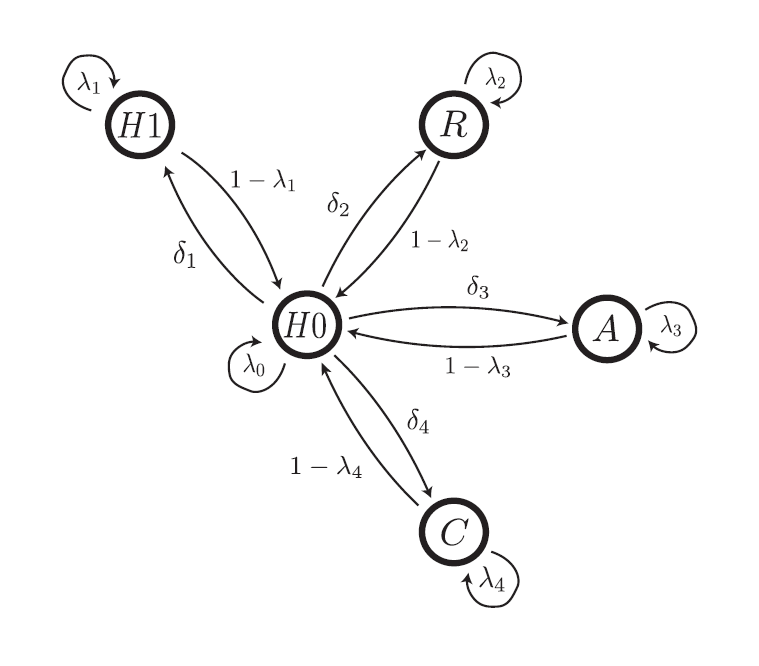
\includegraphics{images/fig_markov_process}}}
  \end{figure}
  
  \begin{equation}\label{eq:stochastic_matrix}
    Pr(s' | s) = A(\vec{\lambda}, \vec{\delta}) = 
    \begin{bmatrix}
      \lambda_0 & \delta_1 & \delta_2 & \delta_3  & \delta_4 \\
      1 - \lambda_1 & \lambda1 & 0 & 0  & 0 \\
      1 - \lambda_2 & 0 & \lambda_2 & 0 & 0 \\
      1 - \lambda_3 & 0 & 0 & \lambda_3  & 0\\
      1 - \lambda_4 & 0 & 0 & 0 & \lambda_4\\
    \end{bmatrix}
  \end{equation}
    
    To summarize, if nature assigns an individual to any health state other than $H0$, our model assumption restricts future events of that individual to two possible outcomes: either she would stay in the current non-$H0$ health state or she would go back to $H0$. This makes $\lambda_i$ the probabilities of an individual staying in the same non-$H0$ health state, and 1 - $\lambda_i$ the probabilities of the individual going back go $H0$.
    
    If nature assigns an individual to heath state $H0$, five possible outcomes could occur: she could transit to the other four health states, $H1$, $R$, $A$, $C$, from $H0$ or she could possibly stay in $H0$. Since the sum of transition probabilities from $H0$ to other four health states plus the probability of staying in $H0$ must be one, there would be a total of five possible outcomes for her in the next period, among which $\lambda_0$ is the probability of staying in $H0$, and $\delta$s are the probabilities of switching to other health states from $H0$.
    
    Once an individual knows her health state, the second stochastic process draws a health care expenditure level from a distribution specific to that particular health state. The following Section \ref{SecEstimation} details the estimation of the Markov transition matrix and examines the state-specific health expenditure processes.


\section{Estimation}\label{SecEstimation}

  We estimate the parameters $\vec{\lambda} = [\lambda_0, \lambda_1, \lambda_2, \lambda_3, \lambda_4]$ and $\vec{\delta} = [\delta_1, \delta_2, \delta_3, \delta_4]$ of the Markov process described in Section \ref{SecModel}. Then, we would use the estimated Markov-process parameters to determine the underlying health state of all positive monthly expenditures. Since the goal of the current section is to test and replicate \citet{evans}, we remain agnostic to the specific characteristics of the five health states, including the three would yield positive health care expenditures. Accordingly, in this section, we use the labels $s \in \{H0, H1, H1, H2, H3\}$ instead of adopting the labels proposed by \citet{evans}.\par
  
  Following \citet{evans}, we assume that the number of consecutive zero expenditure months and the number of consecutive positive expenditure months constitute the principal distinguishing characteristic of health states in the data. We estimate $\vec{\lambda}$ and $\vec{\delta}$ by GMM to match moments that represent the number of consecutive zero health expenditure months as well as the number of consecutive positive health expenditure months.\par
  
  Also, following \citet{evans}, we assume that the proportion of people in each of the five health states is constant over time. Let these proportions be given by a state vector $\textbf{v} = [v_0, v_1, v_2, v_3, v_4]^T$. This ergodic distribution satisfies $\textbf{v}^T\textbf{A} = \textbf{v}^T$. And let $h_{i,t}$ be the monthly health expenditure by individual $i$ in period $t$. Since the two health states $s = \{H0, H1\}$ would always yield zero health care expenditure at period $t$, we can directly compute the probability of 0 health care expenditure in the population at any given time period to be $v_0 + v_1 = Pr(h_{i,t} = 0) = 0.5735$. Therefore, the sum of the estimated values of $H0$ and $H1$ should be closed to 0.5735. \par


\subsection{Estimating Markov process}\label{SecEstimation1}

  We want to know the probabilities of consecutive nonzero health expenditure periods, so we would define $a_k$ to be the probability that an individual had positive expenditure in the current month given that the individual also had positive expenditure in the previous k months. So, probabilistically, $a_k$ is: 
  \begin{equation}\label{eq:ak}
    a_k = Pr(h_{i, t} > 0 | h_{i, t-1} > 0, \dots, h_{i, t-k} > 0)
  \end{equation}
  
  Let $b_k$ represents the unconditional probability that the current period and the previous k periods all had positive expenditure. 
  \begin{equation}\label{eq:bk}
  \begin{split}
    b_k &= Pr(h_{i, t} > 0, h_{i, t-1} > 0, \dots, h_{i, t-k} > 0) \\
        &= Pr(h_{i, t} > 0 | h_{i, t-1} > 0, \dots, h_{i, t-k} > 0) \times
           Pr(h_{i, t-1} > 0, \dots, h_{i, t-k} > 0) \\
        &= a_kb_{k-1} = a_ka_{k-1}b_{k-2} = a_ka_{k-1}a_{k-2}b_{k-3} \\
        &= \prod_{j = 0}^{k} a_j 
            \text{\space \space because \space \space} b_0 = a_0 \\   
  \end{split}
  \end{equation}
  
  By taking the cumulative product of $\{a_j\}_{j = 0}^{k}$ we can determine $\{b_j\}_{j = 0}^{k}$. Notice that the consecutive nonzero claims satisfy the following relations based on our model:
  \begin{equation}\label{eq:bk_cond}
  \begin{split}
    v_2 + v_3 + v_4 &= b_0 \\
    \lambda_2v_2 + \lambda_3v_3 + \lambda_4v_4 &= b_1\\
    \lambda_2^2v_2 + \lambda_3^2v_3 + \lambda_4^2v_4 &= b_1\\
    \lambda_2^3v_2 + \lambda_3^3v_3 + \lambda_4^3v_4 &= b_1\\
    \vdots \\
    \lambda_2^kv_2 + \lambda_3^kv_3 + \lambda_4^kv_4 &= b_1\\      
  \end{split}
  \end{equation}
  
  Analogously for zero expenditures, let $c_k$ be the probability that an individual had zero expenditure in the current month given that the individual also had zero expenditures in the previous $k$ months. So, $c_k$ is: 
  \begin{equation}\label{eq:ck}
    c_k = Pr(h_{i, t} = 0 | h_{i, t-1} = 0, \dots, h_{i, t-k} = 0)
  \end{equation}
  
  We want to know the probabilities of consecutive zero health expenditure periods. Let $d_k$ represent the unconditional probability that the current period and the previous $k$ periods all had zero expenditures.
  \begin{equation}\label{eq:dk}
  \begin{split}
    d_k &= Pr(h_{i, t} = 0, h_{i, t-1} = 0, \dots, h_{i, t-k} = 0) \\
        &= Pr(h_{i, t} = 0 | h_{i, t-1} = 0, \dots, h_{i, t-k} = 0) \times
        Pr(h_{i, t-1} = 0, \dots, h_{i, t-k} = 0) \\
        &= c_kd_{k-1} = c_kc_{k-1}d_{k-2} = c_kc_{k-1}c_{k-2}d_{k-3} \\
        &= \prod_{j = 0}^{k} c_j 
            \text{\space \space because \space \space} d_0 = c_0 \\
  \end{split}
  \end{equation}
  
  By taking the cumulative product of $\{c_j\}_{j = 0}^{k}$ we can determine $\{d_j\}_{j = 0}^{k}$.
  
  The theoretical probabilities of consecutive positive spells in (\ref{eq:bk_cond}) was simple because each spell is defined as being exclusively in one of the positive health states $s = \{R, A, C\}$. However, zero expenditure spells can bounce between the two healthy states $s = \{H0, H1\}$. The theoretical probabilities of consecutive zero claims satisfy the following recursive relation,
  \begin{equation}\label{eq:model_moments}
  \begin{split}
    d_k &= p_{k-1, 0}(\lambda_0 + \delta_1) + p_{k-1, 1}\\
    p_{k, 0} &= p_{k-1, 0}\lambda_0 + p_{k-1, 1}(1 - \lambda_1) \\
    p_{k, 1} &= p_{k-1, 0}\delta_1 + p_{k-1, 1}\lambda_1 \text{\space for \space} k = 1,2,\dots \\
    &\text{\space and \space} d_0 = v_0 + v_1, \text{\space} p_{0, 0} = v_0, \text{\space} p_{0, 1} = v_1 \\  
  \end{split}
  \end{equation}
  where $p_{k,0}$ is the probability of a zero expenditure spell of length $k$ that ends in state $H0$ and $p_{k,1}$ is the probability of a zero expenditure spell of length $k$ that ends in state $H1$. 
  
  Let $\textbf{b} = [b_0, b_1, \dots, b_23]^T$ and $\textbf{d} = [d_0, d_1, \dots, d_23]^T$ be the vectors of data moments to match. We estimate the parameters $\vec{\lambda}$ and $\vec{\delta}$ with the resulting ergodic distribution state vector \textbf{v} by solving the following optimization problem.
  
  \begin{equation}\label{eq:optimization}
  \begin{split}
    \min_{\{\lambda_i\}_{i = 0}^{4}, \{\delta_i\}_{j = 1}^{3}} & \lvert\lvert B(\vec{\lambda})\textbf{v} - \textbf{b} \rvert\rvert_2 + 
    \lvert\lvert D(\vec{\lambda}, \delta_1, \textbf{v}) - \textbf{d} \rvert\rvert_2 \\
    & \text{s.t.} \quad \textbf{v}'A(\vec{\lambda}, \vec{\delta}) = \textbf{v}' \quad
    \text{and} \quad \delta_4 = 1 - \lambda_0 - \delta_1 - \delta_2 - \delta_3\\
    & \text{and} \quad \lambda_i, \delta_j \in (0, 1) \quad \forall i, j
  \end{split}
  \end{equation}

  in which,
  \vspace{6mm}
  \newline
  $B(\vec{\lambda}) =$
  $\begin{bmatrix}
      0 & 0 & 1 & 1 & 1 \\
      0 & 0 & \lambda_2 & \lambda_3 & \lambda_4 \\
      0 & 0 & \lambda_2^2 & \lambda_3^2 & \lambda_4^2 \\
      \vdots & \vdots & \vdots & \vdots & \vdots\\
      0 & 0 & \lambda_2^{T-1} & \lambda_3^{T-1} & \lambda_4^{T-1}\\
  \end{bmatrix}$
  and $D(\vec{\lambda}, \delta_1, \textbf{v}) = $
  $\begin{bmatrix}
      v_0 + v_1 \\
      p_{0, 0}(\lambda_0 + \delta_1) + p_{0, 1} \\
      p_{1, 0}(\lambda_0 + \delta_1) + p_{1, 1} \\
      \vdots \\
      p_{22, 0}(\lambda_0 + \delta_1) + p_{22, 1}\\
  \end{bmatrix}$.
  \vspace{6mm}
    
  \noindent The two norms in (\ref{eq:optimization}) match model moments $B(\vec{\lambda})\textbf{v}$ and $D(\vec{\lambda}, \delta_1, \textbf{v})$ to data moments $\textbf{b}$ and $\textbf{d}$. Also, note that $d_0 = 1 - b_0$. This GMM estimation, therefore, uses 47 moments to estimate 8 parameters.
    
  Table \ref{TabParams} shows the estimates of the $\vec{\lambda}$ and $\vec{\delta}$ Markov probabilities and the implied ergodic distribution $\textbf{v}$. Table \ref{TabMoments} and Figure \ref{Figbkdk} show how closely the estimated model moments $\textbf{b}$ and $\textbf{d}$ match their corresponding data moments. 
  
  \begin{table}[h!] \centering \captionsetup{width=3.0in}
    \caption{\label{TabParams}\textbf{Estimated values of $\vec{\lambda}$ and $\vec{\delta}$ and corresponding $\textbf{v}$}}
      \begin{tabular}{ c c | c  c  c }
      \hline\hline
        & & $\lambda_s$ & $\delta_s$ & $v_s$\\
      \hline
      $H0$ & $s = 0$ & 0.6698 &  & 0.3743 \\
      $H1$ & $s = 1$ & 0.9690 & 0.0167 & 0.2017 \\
      $H2$ & $s = 2$ & 0.8465 & 0.0525 & 0.1281 \\
      $H3$ & $s = 3$ & 0.9796 & 0.0069 & 0.1256 \\
      $H4$ & $s = 4$ & 0.4415 & 0.2541 & 0.1703 \\
      \hline\hline
    \end{tabular}
    % \begin{tablenotes}
    %   \scriptsize{\item[]Note: Maybe put sources here.}
    % \end{tablenotes}
  \end{table}   

  \begin{table}[h!] \centering \captionsetup{width=4.0in}
    \caption{\label{TabMoments}\textbf{Comparison of model moments to data moments}}
      \begin{tabular}{ c c c | c c c | c c c }
      \hline\hline
       & model & data & & model & data & & model & data \\
      \hline
      $b_0$ & 0.4265 & 0.4240 & $b_8$ & 0.1400 & 0.1405 & $b_{16}$ & 0.0996 & 0.0991 \\
      $b_1$ & 0.3014 & 0.3066 & $b_9$ & 0.1326 & 0.1329 & $b_{17}$ & 0.0964 & 0.0959 \\
      $b_2$ & 0.2438 & 0.2455 & $b_{10}$ & 0.1261 & 0.1264 & $b_{18}$ & 0.0935 & 0.0930 \\
      $b_3$ & 0.2106 & 0.2104 & $b_{11}$ & 0.1204 & 0.1206 & $b_{19}$ & 0.0906 & 0.0902 \\
      $b_4$ & 0.1882 & 0.1879 & $b_{12}$ & 0.1152 & 0.1154 & $b_{20}$ & 0.0880 & 0.0877 \\
      $b_5$ & 0.1718 & 0.1718 & $b_{13}$ & 0.1107 & 0.1107 & $b_{21}$ & 0.0855 & 0.0853 \\
      $b_6$ & 0.1591 & 0.1593 & $b_{14}$ & 0.1067 & 0.1065 & $b_{22}$ & 0.0833 & 0.0830 \\
      $b_7$ & 0.1487 & 0.1491 & $b_{15}$ & 0.1030 & 0.1026 & $b_{23}$ & 0.0812 & 0.0809 \\
      \hline\hline
       & model & data & & model & data & & model & data \\
      \hline
      $d_0$ & 0.5735 & 0.5760 & $d_8$ & 0.2072 & 0.2056 & $d_{16}$ & 0.1493 & 0.1522 \\
      $d_1$ & 0.4474 & 0.4587 & $d_9$ & 0.1949 & 0.1955 & $d_{17}$ & 0.1454 & 0.1475 \\
      $d_2$ & 0.3739 & 0.3781 & $d_{10}$ & 0.1848 & 0.1871 & $d_{18}$ & 0.1420 & 0.1431 \\
      $d_3$ & 0.3253 & 0.3222 & $d_{11}$ & 0.1762 & 0.1799 & $d_{19}$ & 0.1387 & 0.1388 \\
      $d_4$ & 0.2893 & 0.2828 & $d_{12}$ & 0.1692 & 0.1734 & $d_{20}$ & 0.1358 & 0.1347 \\
      $d_5$ & 0.2613 & 0.2545 & $d_{13}$ & 0.1633 & 0.1675 & $d_{21}$ & 0.1333 & 0.1307 \\
      $d_6$ & 0.2395 & 0.2337 & $d_{14}$ & 0.1581 & 0.1621 & $d_{22}$ & 0.1310 & 0.1269 \\
      $d_7$ & 0.2217 & 0.2179 & $d_{15}$ & 0.1534 & 0.1570 & $d_{23}$ & 0.1290 & 0.1232 \\
      \hline\hline
    \end{tabular}
    % \begin{tablenotes}
    %   \scriptsize{\item[]Note: Maybe put sources here.}
    % \end{tablenotes}
  \end{table}

  \begin{figure}[h!]\centering \captionsetup{width=4.0in}
    \caption{\label{Figbkdk}\textbf{Plot of $b_k$ and $d_k$ from model versus data for $k = 0, 1, ..., 23$}}
    \fbox{\resizebox{4.0in}{2.7in}{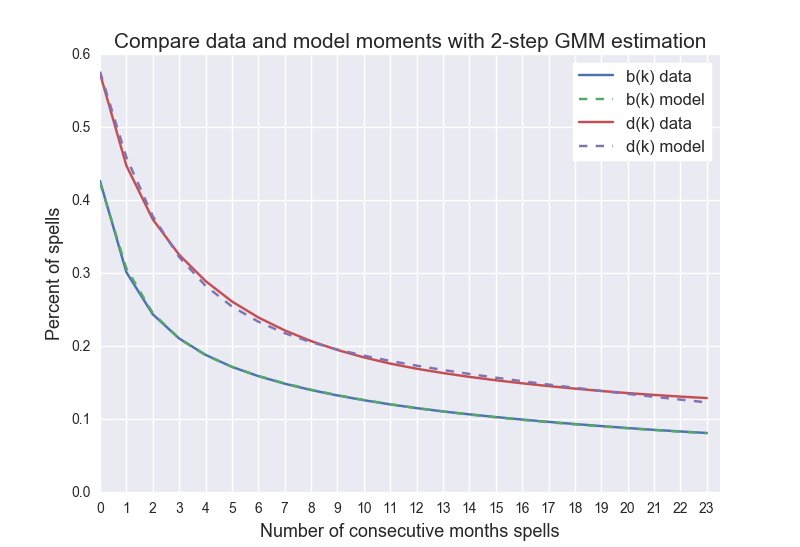
\includegraphics{images/fig_7}}}
  \end{figure}

\subsection{Identifying health expenditure patterns}\label{SecEstimation2}

  Once the parameters for the Markov process $\vec{\lambda}$ and $\vec{\delta}$ and the corresponding ergoticly distributed state matrix $\textbf{v}$ are estimated as in Section \ref{SecEstimation1}, it is now possible to determine the underlying health states $s \in \{H0, H1, H2, H3, H4\}$. Healthy states $s \in \{H0, H1\}$ are represented by zero expenditures months. Accordingly, we can categorize all zero expenditures as either $H0$ or $H1$. On the other hand, each positive expenditure spell of length $n$ has a positive probability of being in any of the three healthy states.\par
  
  Following \citet{evans}, we distinguish four positive expenditure spell types for assigning probabilities of being in three healthy states: 1) spells of $n$ consecutive positive expenditures bounded by a beginning month and an ending month with zero expenditures, 2) front-censored spells that start the sample period with $n$ consecutive positive expenditure months, 3) back-censored spells that end the sample period with $n$ consecutive positive expenditure months, and 4) spells with entire sample having positive expenditures.\par
  
  The probability of each of these four spell types being in any of the positive-expenditure health state are given, in order, by the following four Equations (\ref{eq_uncensored}) through (\ref{eq_2censored}):
  
  \begin{equation} \label{eq_uncensored}
    Pr(h_{i,t} = 0, \{h_{i,j}\}_{j=t-1}^{t-1} > 0, h_{i,t-n-1} = 0) = \sum_{s=2}^4 \delta_s\lambda_s^{n-1} (1 - \lambda_s)  \\
    \text{\space for \space} 1 \leq n \leq 22.
  \end{equation}
    \begin{equation} \label{eq_fcensored}
    Pr(h_{i,n+1} = 0, \{h_{i,j}\}_{j=1}^{n} > 0) = \sum_{s=2}^4 v_s\lambda_s^{n-1} (1 - \lambda_s) \quad \\
    \text{for} \quad 1 \leq n \leq 23.
  \end{equation}
    \begin{equation} \label{eq_bcensored}
    Pr(\{h_{i,j}\}_{j=24-n+1}^{24} > 0, h_{i,24-n} = 0) = \sum_{s=2}^4 \delta_s\lambda_s^{n-1} \quad \text{for} \quad 1 \leq n \leq 23.
  \end{equation}
    \begin{equation} \label{eq_2censored}
    Pr(\{h_{i,j}\}_{j=1}^{n} > 0) = \sum_{s=2}^4 v_s\lambda_s^{n-1} \quad \text{for} \quad n = 24.
  \end{equation}
  
  Figures \ref{Fig_uncensored} and \ref{Fig_2censored} illustrate the probability that a spell of $n$ consecutive positive expenditure is in state $s = \{H2, H3, H4\}$ for both uncensored string type (\ref{eq_uncensored}) and front- and back-censored type (\ref{eq_2censored}) of strings. With the computed probabilities with parameters and ergodic distribution shown in Table \ref{TabParams}, we can determine the underlying health state of each spell of positive expenditure to be the one with the highest probability given the length $n$ and the spell type. For our sample of 2,399,9160 individual monthly expenditures, all front- and back-truncated strings are of length 24 and, therefore, $s = H3$ health-care-consumption type, which is named as $C$ (chronic) type in \citet{evans}. We further stress that our predicted labels for all $n$ for both string types are identical to the predicted labels in \citet{evans}. 

  \begin{figure}[ht!]\centering \captionsetup{width=5.0in}
    \caption{\label{Fig_uncensored}\textbf{Percent probability that uncensored positive expenditure string of length $n$ is type $s$}}
    \fbox{\resizebox{4.0in}{2.7in}{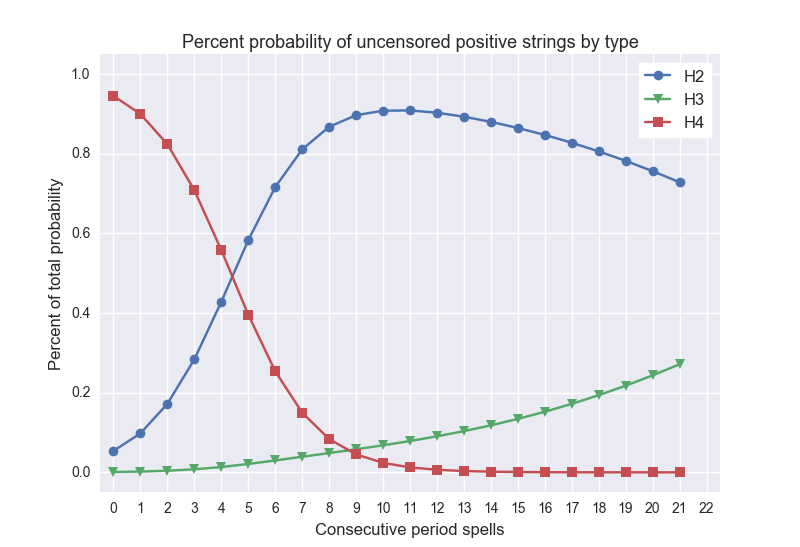
\includegraphics{images/fig_8}}}
  \end{figure}
  \begin{figure}[ht!]\centering \captionsetup{width=5.0in}
    \caption{\label{Fig_2censored}\textbf{Percent probability that front- and back-censored positive expenditure string of length $n$ is type $s$}}
    \fbox{\resizebox{4.0in}{2.7in}{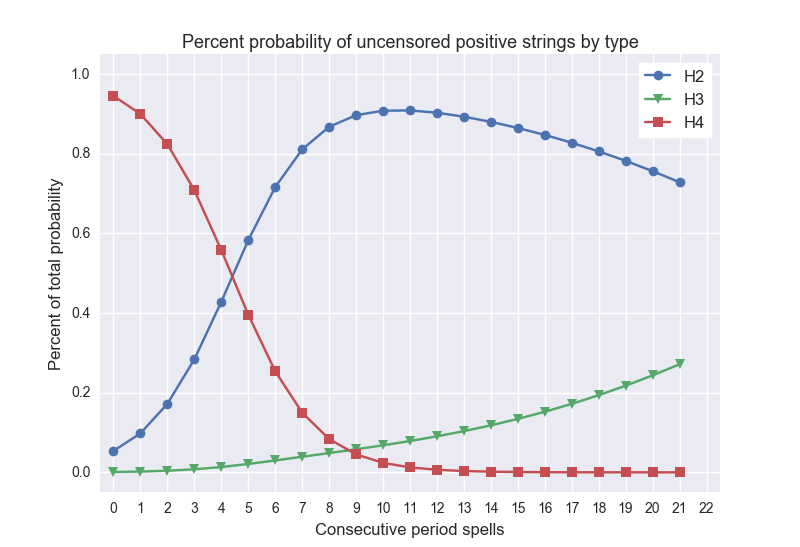
\includegraphics{images/fig_8}}}
  \end{figure}
  
  We now explore and examine the characteristics of the three health states determined by the spell length and type of positive expenditures. Table \ref{TabExpPatterns} summarizes the characteristics of the positive expenditure of all three health states across gender and age dimensions. Individuals are divided into four age groups: younger than than 21 years old, between 21 to 44 years old, between 45 to 64 years old, and older than 65 years old. Although largely arbitrary and with little theoretical justification, our division of age groups serves adequately the purpose of this section, which is exploratory in nature. 

 \begin{table}[h!] \centering \captionsetup{width=4.0in}
    \caption{\label{TabExpPatterns}\textbf{Comparison of positive expenditure patterns across gender and age}}
      \begin{tabular}{ c c | c c c c }
        \hline\hline
         & & $H2$ & $H3$ & $H4$ & Total \\ 
        \hline
        Count & All & 277,056 & 283,213 & 462,916 & 1,023,185\\
        & Female  & 164,017 & 169,934 & 250,234 & 584,185 \\
        & Male & 113,039 & 113,279 & 212,682 & 439,000 \\
        & Age ($<21$) & 50,216  & 27,231 & 164,519 & 241,966 \\
        & Age ($<45$) & 101,061  & 82,189 &  153,296 & 336,546 \\ 
        & Age ($<65$) & 119,435 & 161,555 & 139,454 & 420,444 \\ 
        & Age ($\geq65$) & 6,344 & 12,238 & 5,647 & 24,229 \\ 
        \hline
        Mean & All & 798.71 & 1,073.61 & 447.46 & 715.88 \\ 
        & Female  & 753.09 & 1,010.54 & 431.79 & 690.35 \\ 
        & Male & 864.89 & 1,168.23 & 465.89 & 749.86 \\ 
        & Age ($<21$) & 605.37 & 1,107.95 & 342.77 & 483.38 \\ 
        & Age ($<45$) & 742.09 & 859.14 & 486.15 & 654.09 \\ 
        & Age ($<65$) & 917.64 & 1,157.64 & 520.78 & 878.23 \\ 
        & Age ($\geq65$) & 991.94 & 1,328.38 & 636.15 & 1078.95 \\ 
        \hline
        St. Dev. & All & 3,771.12 & 4,650.51 & 1,833.88 & 3,380.62\\
        & Female & 3,059.81 & 3,897.57 & 1,625.46 & 2,859.95\\ 
        & Male & 4,611.30 & 5,591.74 & 2,052.03 & 3,947.60 \\
        & Age ($<21$) & 3,606.08 & 6,251.56 & 1,538.57 & 2,950.69\\
        & Age ($<45$) & 3,212.72 & 3,741.47 & 1,893.12 & 2,735.59\\
        & Age ($<65$) & 4,232.99 & 4,731.42 & 1,999.29 & 3,875.27\\
        & Age ($\geq65$) & 3,966.34 & 4,851.03 & 3,193.50 & 4,287.45\\
        \hline\hline
    \end{tabular}
    % \begin{tablenotes}
    %   \scriptsize{\item[]Note: Maybe put sources here.}
    % \end{tablenotes}
  \end{table}

  Table \ref{TabExpPatterns} shows that $H4$ is the most common expenditure type in general, except for the over-65-year-old age group for which the most common type is $H3$ (50.51\%). In fact, the proportion of $H3$ type expenditures increase with age (12.67\% for the youngest age group, 24.42\% for the next age group, and 38.42\% for the third age group). Between male and female, monthly health expenditures by male individuals are more likely to be of $H4$ type (48.45\%) than health expenditures by female individuals (42.83\%). On the other hand, on average, the most expensive expenditure type is $H3$, the second most expenditure type is $H2$, and the least expensive is $H4$ for the entire sample as well as all subgroups. The same pattern holds for the standard deviation of monthly health expenditure across $s = \{H2, H3, H4\}$. That is, $H3$ is the most expensive expenditure type with the greatest variance. $H2$ is the next most expensive type with the second greatest variance. $H4$ is the least expensive type of health expenditure with the smallest variance.\par
  
  This, then, leads to our evaluation of the original labels by \citet{evans}, namely, $s = \{R, C, A\}$. The comparison of percent probabilities that the positive expenditure string of varying $n$ is of type $s$ between the original study and ours suggests that $R$ (regular), $C$ (chronic), and $A$ (acute) corresponds to our $H4$, $H3$, and $H2$, respectively. We observe that $R$ type expenditures are generally the most common type with the lowest mean and standard deviation. Figure \ref{Fig_uncensored} also shows that $R$ type of expenditures have shorter spells other expenditure types. This is also true in cases of front-censored spells and back-censored spells. $C$ type expenditures are more common among older than 65-year-old group and the largest in mean and standard deviation. In addition, $C$ type of expenditure spells consist of at least 13 consecutive months. As Figure \ref{Fig_2censored} shows, all expenditure spells of 24 consecutive months are $C$ type. Finally, $A$ type expenditures appear as a middle stage between the of $R$ and $C$ types in terms of proportion, mean, standard deviation and spell length.
  
  Based on this evaluation, we suggest that the original labels may not be the most appropriate for the corresponding positive health care expenditure patterns. For example, the spell length $n$ for $A$ (acute) type, which can extend up to 23 consecutive month (See Figure \ref{Fig_uncensored}) may not fit the medical usages of the term ``acute''.\footnote{For example, the ``acute illness'' entry in \citet{med} states that the term denotes ``a serious illness that appears suddenly but usually does not last lon''g. This does not seem to best characterize $H2$ health-care-consumption state, which has the positive expenditure spell length of 6 to 23 months.} In addition, $R$ for ``regular'' health-care-consumption state may misrepresent the underlying health condition of an individual characterized by a short-term (i.e., 1 to 5 consecutive months) positive health expenditure. Therefore, we propose an alternative labeling scheme for positive expenditure types $s = \{M, S, C\}$, where $M$ denotes ``moderately ill'', $S$ denotes ``severely ill'', and $C$ denotes ``chronically ill''. $M$, $S$, and $C$ in our proposal corresponds to $R$, $A$, and $C$ in the original study, respectively.
     
  
\section{Conclusion}\label{SecConclusion}

  This paper replicates and evaluates a Markov regime-switching approach to estimating individual health care cost dynamics first proposed by \citet{evans}. Using the GMM procedure for estimating model parameters as described in the original study, we successfully match the targeted moments to an impressive degree of precision. The model, however, appears sensitive to initial parameter guesses. We also validate the existence of the three distinct types of health care consumption. The estimated probabilities that a truncated or non-truncated string of $n$ consecutive positive expenditure is of a specific health state $s \in \{H2, H3, H4\}$ allow us to label each spell of positive health expenditures. We examine and compare the characteristics of the labelled expenditures with gender and age variables. Our examination suggests that the original labelling scheme of $R$ for regular health-care-consumption state, $C$ for chronic health-care-consumption state, and $A$ for acute health-care-consumption state potentially misrepresents the empirical characteristics of three positive health expenditure states. We then propose an alternative labeling scheme, in which  $M$ represents ``moderately ill'', $S$ represents ``severely ill'', and $C$ represents ``chronically ill''.

  \clearpage


\end{spacing}


\newpage
\bibliographystyle{plainnat}
\bibliography{citation}


\newpage
\renewcommand{\theequation}{A.\arabic{section}.\arabic{equation}}
                                                 % redefine the command that creates the section number
\renewcommand{\thesection}{A-\arabic{section}}   % redefine the command that creates the equation number
\setcounter{equation}{0}                         % reset counter
\setcounter{section}{0}                          % reset section number
\end{document}